\documentclass{article}

\usepackage[utf8]{inputenc}

\usepackage{mathtools}
\usepackage{amsmath}
\usepackage{amssymb}

\usepackage{graphicx}

\usepackage{algpseudocode}
\usepackage{algorithmicx}

\title{Numerical Implementation of the Natural Exponential}
\author{Alberte Mørk}
\date{}

\begin{document}

\maketitle

There are several ways of defining the natural exponential, $\exp(x)$. One could define it as the solution of the differential equation $y' = y$ or as the limit $\lim_{n \rightarrow \infty} (1 + x/n)^n$. They all turn out to be equal. The most common way, and the way most relavant for our purpose, is by the power series, 
%
\begin{align*}
	\exp (x) \coloneqq \sum_{k = 0}^\infty \frac{x^k}{k!}.
\end{align*}
%
With a bit of knowledge of complex function theory it is rather straightforward to show that the convergence radius of this function is infinite, making the function well-defined on all of $\mathbb{C}$. 

The definition is handy in the framework of numerics is because it only consists of basis operations addition and multiplication. To exploit this feature, we rewrite the sum as
%
\begin{align*}
	\exp (x) = 1 + x \left( 1 + \frac{x}{2} \left( 1 + \frac{x}{3} \left( \dots \right) \right) \right).
\end{align*}
%
By making this rewriting we avoid power functions, which are slower than ordinary multiplication. Another perk is that the computer will start the calculation from the innermost bracket, such that the smallest contributions are calculated first. This becomes a problem for negative values, as these will have the largest contribution first. To overcome this issue, we define the function recursively to return the inverse of the function taken on the positive value if the input is negative. 
%
\begin{algorithmic}
	\If {$x < 0$}
	\Return $\frac{1}{\exp(-x)}$
	\EndIf
\end{algorithmic}

The next issue that arises, is the fact that we cannot start at infinity. This we adress by noting that for small input values, the higher order terms are negligibly small. To ensure that the argument is small we implement another recursive algoritm. 
%
\begin{algorithmic}
	\If {$x < \epsilon$}
	\Return $\exp \left( \frac{x}{2} \right)^2$
	\EndIf
\end{algorithmic}
%
The value $\epsilon$ is chosen to be small. For higher precision, lower values of $\epsilon$ is used. This finally allows us to define the function 
%
\begin{algorithmic}
	\Function{$\exp$}{$x$}
	\If {$x < 0$}
	\Return $\frac{1}{\exp(-x)}$
	\EndIf
	\If {$x < \epsilon$}
	\Return $\exp \left( \frac{x}{2} \right)^2$
	\EndIf
	\Return $1 + x\left( 1 + \frac{x}{2} \left( \text{to order } n \right) \right)$
	\EndFunction
\end{algorithmic}

We have made a specific implementation usign $\epsilon = 1/8$ and $n = 10$. This gives us the plot below, which shows a good correspondence between the numerical rutines, and the rutine from math.h. 
%
\begin{center}
	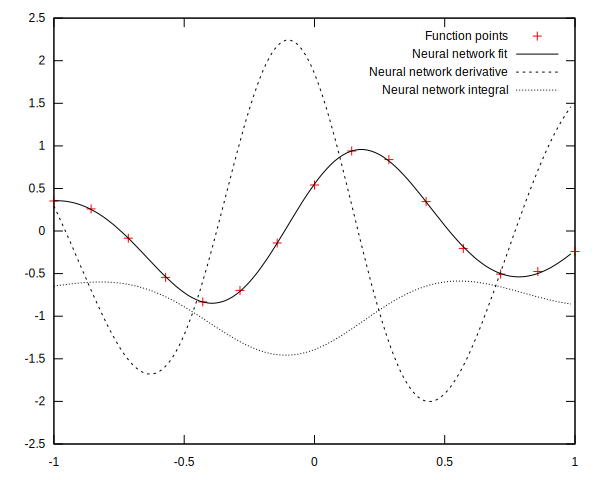
\includegraphics[width = \columnwidth]{plot.png}
\end{center}


\end{document}
